\begin{enumerate}
    \item
    Từ hình \ref{fig:41}, ta có thể dễ dàng chỉ ra được phương và chiều của đường sức từ như hình \ref{fig:43}. \\

    Áp dụng quy tắc bàn tay trái: Đặt bàn tay sao cho ngón tró chỉ vào màn hình, lòng bàn tay hướng sao để nhận được các đường sức từ vuông góc với mặt bàn tay. Ngón cái duỗi thẳng ra sẽ là chiều của lực điện từ, được mô tả như hình \ref{fig:43}. \\

    \textbf{Bình luận}: Bằng các kiến thức về trường điện từ, động lực học và động lực học tương đối tính, ta có thể  để giải thích về quỹ đạo của hạt khi đi vào tứ cực từ. Cụ thể, trên phương $y$, do lực điện từ luôn hướng vào tâm của tứ cực từ nên hạt sẽ bị \textbf{hội tụ}. Tương tự, trên phương $x$, lực điện từ đều hướng ra xa tâm của tứ cực từ nên hạt sẽ bị \textbf{phân kì}. 
    
    \begin{figure}[!ht]
    \centering
    \scalebox{0.82}{
    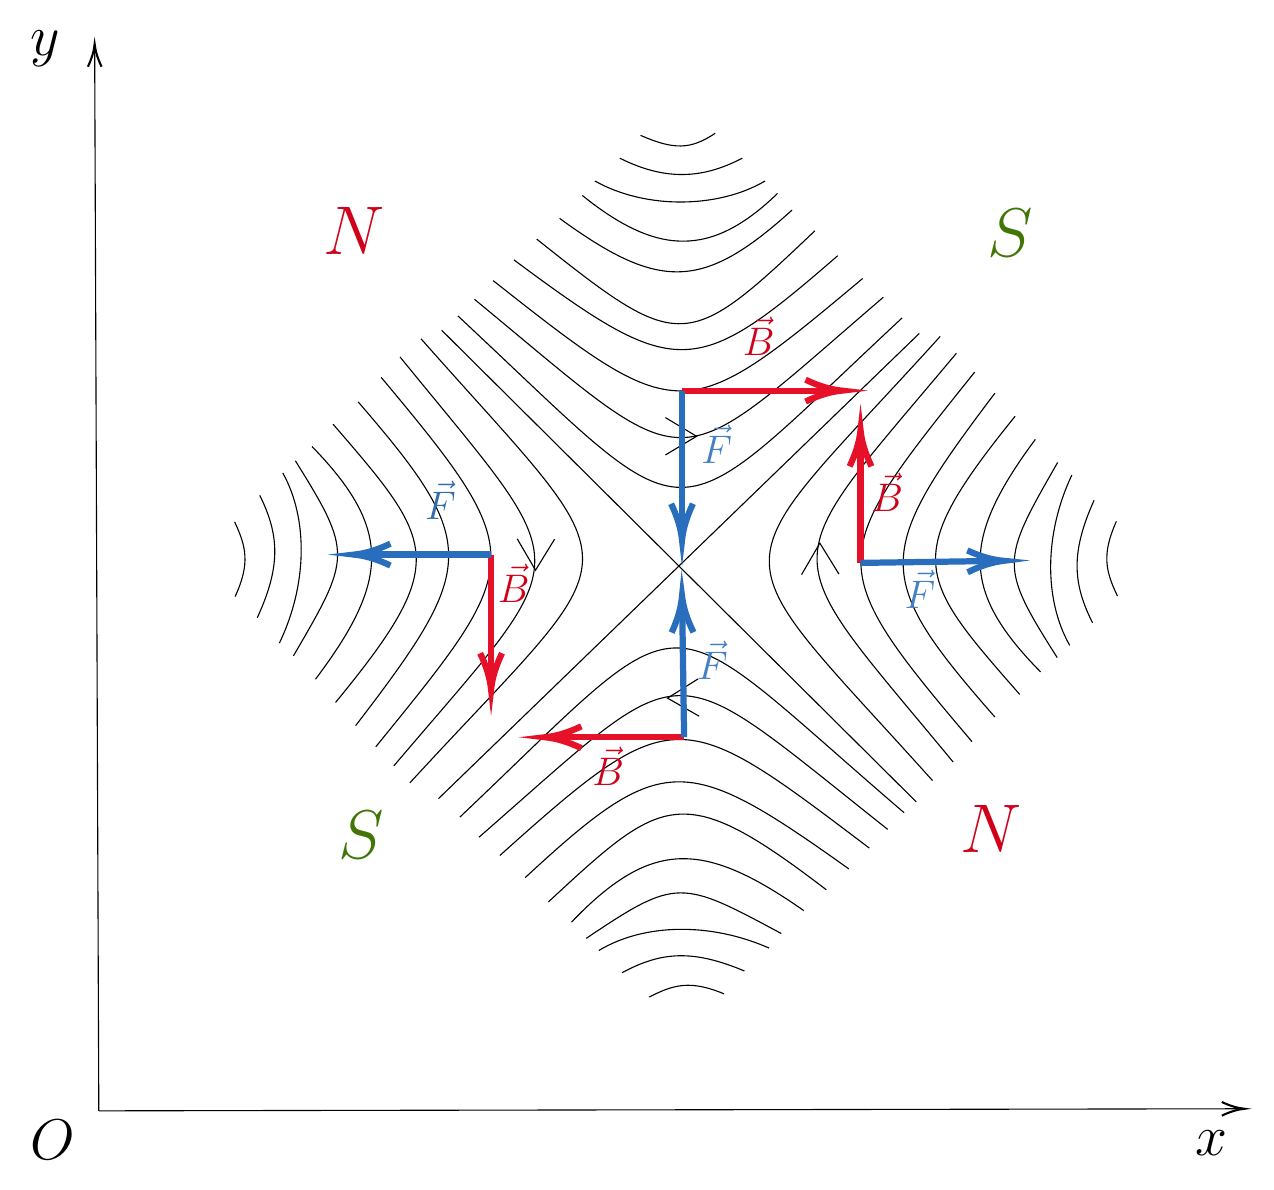
\begin{tikzpicture}[x=0.75pt,y=0.75pt,yscale=-1,xscale=1]
        %uncomment if require: \path (0,642); %set diagram left start at 0, and has height of 642
        
        %Curve Lines [id:da4792522475831378] 
        \draw    (266,156) .. controls (356,227) and (358,227) .. (444,155) ;
        %Curve Lines [id:da18776678628173316] 
        \draw    (257,165) .. controls (365,254) and (349,254) .. (454,164) ;
        %Curve Lines [id:da7579049508332776] 
        \draw    (249,173) .. controls (367,283) and (346,283) .. (463,174) ;
        %Curve Lines [id:da9068961265681277] 
        \draw    (276,146) .. controls (354,204) and (363,204) .. (432,144) ;
        %Curve Lines [id:da6057096352515956] 
        \draw    (287,136) .. controls (356,191) and (359,191) .. (421,132) ;
        %Curve Lines [id:da6124834939512256] 
        \draw    (298,126) .. controls (346,161) and (367,161) .. (410,122) ;
        %Curve Lines [id:da999176140900975] 
        \draw    (309,115) .. controls (345,144) and (371,145) .. (403,114) ;
        %Curve Lines [id:da4412765595880592] 
        \draw    (315,108) .. controls (340,122) and (375,121) .. (397,108) ;
        %Curve Lines [id:da6165862171426286] 
        \draw    (327,97) .. controls (349,108) and (367,107) .. (386,97) ;
        %Curve Lines [id:da5352330674257251] 
        \draw    (337,86) .. controls (353,93) and (361,93) .. (373,85) ;
        %Straight Lines [id:da13696112022895202] 
        \draw    (241.18,179.89) -- (469.82,407.11) ;
        %Straight Lines [id:da612929119766775] 
        \draw    (239.67,405.57) -- (471.33,181.43) ;
        %Curve Lines [id:da9013347475427187] 
        \draw    (209.43,380.62) .. controls (281.45,292.07) and (284.48,289.13) .. (212.07,202.64) ;
        %Curve Lines [id:da8829915710419369] 
        \draw    (218.14,389.8) .. controls (308.32,283.62) and (308,299.62) .. (221.17,192.82) ;
        %Curve Lines [id:da839350917569065] 
        \draw    (225.88,397.96) .. controls (335.11,279.16) and (336.6,303.2) .. (231.24,184.02) ;
        %Curve Lines [id:da09708382750689237] 
        \draw    (199.74,370.42) .. controls (258.67,293.61) and (259.88,282.63) .. (200.95,214.41) ;
        %Curve Lines [id:da6233083389607426] 
        \draw    (190.08,359.22) .. controls (245.86,291.35) and (238.14,282.19) .. (188.87,225.17) ;
        %Curve Lines [id:da9303172125407404] 
        \draw    (180.42,348.02) .. controls (216,300.74) and (217.5,275.76) .. (178.76,235.96) ;
        %Curve Lines [id:da2769813795168756] 
        \draw    (169.77,336.8) .. controls (197.44,289.36) and (198.47,287.38) .. (170.71,242.8) ;
        %Curve Lines [id:da812357712173224] 
        \draw    (162.98,330.66) .. controls (176.4,302.93) and (177.05,270.94) .. (164.65,248.68) ;
        %Curve Lines [id:da730462575275286] 
        \draw    (152.35,318.44) .. controls (163.73,293.67) and (163.05,278.65) .. (153.55,259.45) ;
        %Curve Lines [id:da735579584390504] 
        \draw    (141.68,308.22) .. controls (148.93,292.37) and (147.11,284.33) .. (141.43,272.21) ;
        
        %Curve Lines [id:da9957314369504402] 
        \draw    (447.23,429.41) .. controls (356.24,360.51) and (353.19,357.59) .. (269.26,432.95) ;
        %Curve Lines [id:da42061516499279983] 
        \draw    (456.1,420.39) .. controls (346.85,333.94) and (362.85,333.72) .. (259.14,424.19) ;
        %Curve Lines [id:da6302289013179545] 
        \draw    (463.99,412.36) .. controls (341.47,307.32) and (365.44,305) .. (250,414.44) ;
        %Curve Lines [id:da6314722799353274] 
        \draw    (437.37,439.44) .. controls (358.56,383.22) and (347.55,382.39) .. (281.42,443.65) ;
        %Curve Lines [id:da7627601342878407] 
        \draw    (426.52,449.49) .. controls (356.74,396.1) and (347.86,404.14) .. (292.59,455.36) ;
        %Curve Lines [id:da5517437382717942] 
        \draw    (415.66,459.53) .. controls (367.17,425.61) and (342.16,424.98) .. (303.73,465.09) ;
        %Curve Lines [id:da2523109982366758] 
        \draw    (404.82,470.56) .. controls (356.44,444.56) and (354.42,443.6) .. (310.84,472.9) ;
        %Curve Lines [id:da5531448424788401] 
        \draw    (398.92,477.57) .. controls (370.73,465.12) and (338.74,465.57) .. (316.92,478.74) ;
        %Curve Lines [id:da8274878407169837] 
        \draw    (387.07,488.61) .. controls (361.92,478.1) and (346.93,479.3) .. (328.08,489.46) ;
        %Curve Lines [id:da2516778847803036] 
        \draw    (377.23,499.63) .. controls (361.13,492.94) and (353.16,495.03) .. (341.25,501.14) ;
        
        %Curve Lines [id:da44567985870338966] 
        \draw    (497.97,200.1) .. controls (426.63,289.2) and (423.63,292.16) .. (496.69,378.1) ;
        %Curve Lines [id:da18107514459279583] 
        \draw    (489.19,190.99) .. controls (399.82,297.86) and (400.03,281.86) .. (487.67,387.99) ;
        %Curve Lines [id:da3520275384011575] 
        \draw    (481.38,182.89) .. controls (373.06,302.52) and (371.39,278.5) .. (477.67,396.86) ;
        %Curve Lines [id:da5409134618202889] 
        \draw    (507.73,210.23) .. controls (449.39,287.49) and (448.27,298.48) .. (507.72,366.24) ;
        %Curve Lines [id:da5658457580650191] 
        \draw    (517.48,221.35) .. controls (462.22,289.65) and (470.02,298.75) .. (519.72,355.39) ;
        %Curve Lines [id:da41437201980134053] 
        \draw    (527.22,232.48) .. controls (492.01,280.03) and (490.7,305.02) .. (529.75,344.52) ;
        %Curve Lines [id:da607470080861005] 
        \draw    (537.96,243.62) .. controls (510.65,291.27) and (509.64,293.26) .. (537.75,337.62) ;
        %Curve Lines [id:da3226182027720166] 
        \draw    (544.8,249.7) .. controls (531.59,277.54) and (531.18,309.53) .. (543.76,331.7) ;
        %Curve Lines [id:da59845594322587] 
        \draw    (555.52,261.84) .. controls (544.33,286.7) and (545.13,301.71) .. (554.77,320.84) ;
        %Curve Lines [id:da3781492316292461] 
        \draw    (566.27,271.98) .. controls (559.15,287.89) and (561.02,295.91) .. (566.8,307.99) ;
        
        %Straight Lines [id:da8548346448041899] 
        \draw    (76,556) -- (74.01,44) ;
        \draw [shift={(74,42)}, rotate = 89.78] [color={rgb, 255:red, 0; green, 0; blue, 0 }  ][line width=0.75]    (10.93,-3.29) .. controls (6.95,-1.4) and (3.31,-0.3) .. (0,0) .. controls (3.31,0.3) and (6.95,1.4) .. (10.93,3.29)   ;
        %Straight Lines [id:da8984436400560898] 
        \draw    (76,556) -- (626,555) ;
        \draw [shift={(628,555)}, rotate = 179.9] [color={rgb, 255:red, 0; green, 0; blue, 0 }  ][line width=0.75]    (10.93,-3.29) .. controls (6.95,-1.4) and (3.31,-0.3) .. (0,0) .. controls (3.31,0.3) and (6.95,1.4) .. (10.93,3.29)   ;
        \draw   (349,222) -- (364,231) -- (349,240) ;
        \draw   (295.58,280.6) -- (286.41,295.5) -- (277.59,280.4) ;
        \draw   (365.2,365.83) -- (350,357.16) -- (364.8,347.84) ;
        \draw   (414.6,297.62) -- (423.4,282.5) -- (432.6,297.38) ;
        %Straight Lines [id:da6158567950762239] 
        \draw [color={rgb, 255:red, 231; green, 16; blue, 41 }  ,draw opacity=1 ][line width=2.25]    (357,209) -- (430,209) ;
        \draw [shift={(434,209)}, rotate = 180] [color={rgb, 255:red, 231; green, 16; blue, 41 }  ,draw opacity=1 ][line width=2.25]    (17.49,-5.26) .. controls (11.12,-2.23) and (5.29,-0.48) .. (0,0) .. controls (5.29,0.48) and (11.12,2.23) .. (17.49,5.26)   ;
        %Straight Lines [id:da4424105608351112] 
        \draw [color={rgb, 255:red, 231; green, 16; blue, 41 }  ,draw opacity=1 ][line width=2.25]    (265,288) -- (265,349) ;
        \draw [shift={(265,353)}, rotate = 270] [color={rgb, 255:red, 231; green, 16; blue, 41 }  ,draw opacity=1 ][line width=2.25]    (17.49,-5.26) .. controls (11.12,-2.23) and (5.29,-0.48) .. (0,0) .. controls (5.29,0.48) and (11.12,2.23) .. (17.49,5.26)   ;
        %Straight Lines [id:da6470847365790864] 
        \draw [color={rgb, 255:red, 231; green, 16; blue, 41 }  ,draw opacity=1 ][line width=2.25]    (358,376) -- (295,376) ;
        \draw [shift={(291,376)}, rotate = 360] [color={rgb, 255:red, 231; green, 16; blue, 41 }  ,draw opacity=1 ][line width=2.25]    (17.49,-5.26) .. controls (11.12,-2.23) and (5.29,-0.48) .. (0,0) .. controls (5.29,0.48) and (11.12,2.23) .. (17.49,5.26)   ;
        %Straight Lines [id:da3950467179843975] 
        \draw [color={rgb, 255:red, 231; green, 16; blue, 41 }  ,draw opacity=1 ][line width=2.25]    (443,292) -- (443,232) ;
        \draw [shift={(443,228)}, rotate = 90] [color={rgb, 255:red, 231; green, 16; blue, 41 }  ,draw opacity=1 ][line width=2.25]    (17.49,-5.26) .. controls (11.12,-2.23) and (5.29,-0.48) .. (0,0) .. controls (5.29,0.48) and (11.12,2.23) .. (17.49,5.26)   ;
        %Straight Lines [id:da6524626189189908] 
        \draw [color={rgb, 255:red, 41; green, 109; blue, 189 }  ,draw opacity=1 ][line width=2.25]    (357,209) -- (357,277) ;
        \draw [shift={(357,281)}, rotate = 270] [color={rgb, 255:red, 41; green, 109; blue, 189 }  ,draw opacity=1 ][line width=2.25]    (17.49,-5.26) .. controls (11.12,-2.23) and (5.29,-0.48) .. (0,0) .. controls (5.29,0.48) and (11.12,2.23) .. (17.49,5.26)   ;
        %Straight Lines [id:da254755616957272] 
        \draw [color={rgb, 255:red, 41; green, 109; blue, 189 }  ,draw opacity=1 ][line width=2.25]    (265,288) -- (203,288) ;
        \draw [shift={(199,288)}, rotate = 360] [color={rgb, 255:red, 41; green, 109; blue, 189 }  ,draw opacity=1 ][line width=2.25]    (17.49,-5.26) .. controls (11.12,-2.23) and (5.29,-0.48) .. (0,0) .. controls (5.29,0.48) and (11.12,2.23) .. (17.49,5.26)   ;
        %Straight Lines [id:da23858917121242795] 
        \draw [color={rgb, 255:red, 41; green, 109; blue, 189 }  ,draw opacity=1 ][line width=2.25]    (358,376) -- (357.06,312) ;
        \draw [shift={(357,308)}, rotate = 89.16] [color={rgb, 255:red, 41; green, 109; blue, 189 }  ,draw opacity=1 ][line width=2.25]    (17.49,-5.26) .. controls (11.12,-2.23) and (5.29,-0.48) .. (0,0) .. controls (5.29,0.48) and (11.12,2.23) .. (17.49,5.26)   ;
        %Straight Lines [id:da12409381028031974] 
        \draw [color={rgb, 255:red, 41; green, 109; blue, 189 }  ,draw opacity=1 ][line width=2.25]    (443,292) -- (508,291.06) ;
        \draw [shift={(512,291)}, rotate = 179.17] [color={rgb, 255:red, 41; green, 109; blue, 189 }  ,draw opacity=1 ][line width=2.25]    (17.49,-5.26) .. controls (11.12,-2.23) and (5.29,-0.48) .. (0,0) .. controls (5.29,0.48) and (11.12,2.23) .. (17.49,5.26)   ;
        
        % Text Node
        \draw (183,119.4) node [anchor=north west][inner sep=0.75pt]  [font=\Huge,color={rgb, 255:red, 208; green, 2; blue, 27 }  ,opacity=1 ]  {$N$};
        % Text Node
        \draw (490,407.4) node [anchor=north west][inner sep=0.75pt]  [font=\Huge,color={rgb, 255:red, 208; green, 2; blue, 27 }  ,opacity=1 ]  {$N$};
        % Text Node
        \draw (503,120.4) node [anchor=north west][inner sep=0.75pt]  [font=\Huge,color={rgb, 255:red, 65; green, 117; blue, 5 }  ,opacity=1 ]  {$S$};
        % Text Node
        \draw (190,410.4) node [anchor=north west][inner sep=0.75pt]  [font=\Huge,color={rgb, 255:red, 65; green, 117; blue, 5 }  ,opacity=1 ]  {$S$};
        % Text Node
        \draw (42,559.4) node [anchor=north west][inner sep=0.75pt]  [font=\huge]  {$O$};
        % Text Node
        \draw (603,564.4) node [anchor=north west][inner sep=0.75pt]  [font=\huge]  {$x$};
        % Text Node
        \draw (42,34.4) node [anchor=north west][inner sep=0.75pt]  [font=\huge]  {$y$};
        % Text Node
        \draw (385,172.4) node [anchor=north west][inner sep=0.75pt]  [font=\Large,color={rgb, 255:red, 208; green, 2; blue, 27 }  ,opacity=1 ]  {$\vec{B}$};
        % Text Node
        \draw (267,291.4) node [anchor=north west][inner sep=0.75pt]  [font=\Large,color={rgb, 255:red, 208; green, 2; blue, 27 }  ,opacity=1 ]  {$\vec{B}$};
        % Text Node
        \draw (312.5,379.4) node [anchor=north west][inner sep=0.75pt]  [font=\Large,color={rgb, 255:red, 208; green, 2; blue, 27 }  ,opacity=1 ]  {$\vec{B}$};
        % Text Node
        \draw (447,247.4) node [anchor=north west][inner sep=0.75pt]  [font=\Large,color={rgb, 255:red, 208; green, 2; blue, 27 }  ,opacity=1 ]  {$\vec{B}$};
        % Text Node
        \draw (365,224.4) node [anchor=north west][inner sep=0.75pt]  [font=\Large,color={rgb, 255:red, 68; green, 128; blue, 196 }  ,opacity=1 ]  {$\vec{F}$};
        % Text Node
        \draw (232,251.4) node [anchor=north west][inner sep=0.75pt]  [font=\Large,color={rgb, 255:red, 50; green, 108; blue, 170 }  ,opacity=1 ]  {$\vec{F}$};
        % Text Node
        \draw (363,328.4) node [anchor=north west][inner sep=0.75pt]  [font=\Large,color={rgb, 255:red, 68; green, 128; blue, 196 }  ,opacity=1 ]  {$\vec{F}$};
        % Text Node
        \draw (463,294.4) node [anchor=north west][inner sep=0.75pt]  [font=\Large,color={rgb, 255:red, 68; green, 128; blue, 196 }  ,opacity=1 ]  {$\vec{F}$};


    \end{tikzpicture}
    } \\
    \caption{Đường sức từ và lực điện từ của tứ cực từ}
    \label{fig:43}
    \end{figure}

    \item
    \begin{enumerate}
    \item 
    Chọn trục chính hướng theo phương $z$ và đi qua gốc tọa độ $O$, ta có thể vẽ được đường đi của hạt trên phương $x$ và $y$ như hình \ref{fig:44}. \\

    Sử dụng các cặp tam giác đồng dạng khác nhau, ta sẽ thu về được hai phương trình tỉ lệ:

    \begin{equation}
        \begin{cases}
        \
        \begin{alignedat}{2}
            & \frac{x_0}{f} = \frac{x}{L+f}
            \\
            & \frac{y_0}{f} = \frac{y}{f-L}
        \end{alignedat}
        \end{cases}
        \iff
        \begin{cases}
        \
        \begin{alignedat}{2}
            & x =\frac{x_0(L+f)}{f}.
            \\
            & y = \frac{y_0 (f-L)}{f}.
        \end{alignedat}
        \end{cases}
    \end{equation}
    
        \begin{figure}[!ht]
        \centering
        \scalebox{0.75}{
        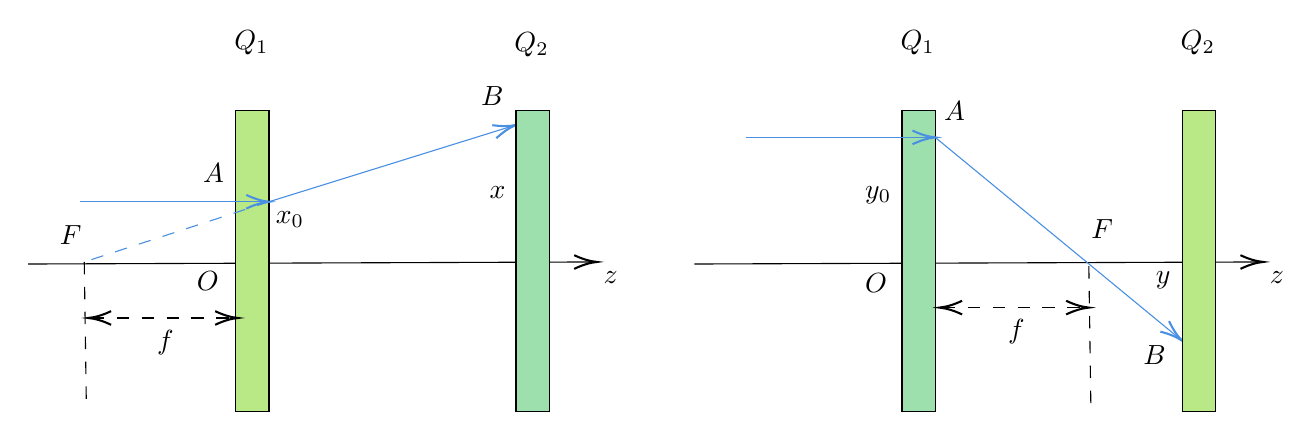
\begin{tikzpicture}[x=0.75pt,y=0.75pt,yscale=-1,xscale=1]
        %uncomment if require: \path (0,300); %set diagram left start at 0, and has height of 300
        
        %Straight Lines [id:da7173986434372925] 
        \draw    (29,151) -- (301,150.01) ;
        \draw [shift={(303,150)}, rotate = 179.79] [color={rgb, 255:red, 0; green, 0; blue, 0 }  ][line width=0.75]    (10.93,-3.29) .. controls (6.95,-1.4) and (3.31,-0.3) .. (0,0) .. controls (3.31,0.3) and (6.95,1.4) .. (10.93,3.29)   ;
        %Shape: Rectangle [id:dp9625003494297018] 
        \draw  [fill={rgb, 255:red, 184; green, 233; blue, 134 }  ,fill opacity=1 ] (129,77) -- (145,77) -- (145,222) -- (129,222) -- cycle ;
        %Straight Lines [id:da10036632412285429] 
        \draw [color={rgb, 255:red, 74; green, 144; blue, 226 }  ,draw opacity=1 ]   (54,121) -- (143,121) ;
        \draw [shift={(145,121)}, rotate = 180] [color={rgb, 255:red, 74; green, 144; blue, 226 }  ,draw opacity=1 ][line width=0.75]    (10.93,-3.29) .. controls (6.95,-1.4) and (3.31,-0.3) .. (0,0) .. controls (3.31,0.3) and (6.95,1.4) .. (10.93,3.29)   ;
        %Straight Lines [id:da3075592337273678] 
        \draw [color={rgb, 255:red, 74; green, 144; blue, 226 }  ,draw opacity=1 ]   (145,121) -- (262.09,84.59) ;
        \draw [shift={(264,84)}, rotate = 162.73] [color={rgb, 255:red, 74; green, 144; blue, 226 }  ,draw opacity=1 ][line width=0.75]    (10.93,-3.29) .. controls (6.95,-1.4) and (3.31,-0.3) .. (0,0) .. controls (3.31,0.3) and (6.95,1.4) .. (10.93,3.29)   ;
        %Straight Lines [id:da9053908768036041] 
        \draw [color={rgb, 255:red, 74; green, 144; blue, 226 }  ,draw opacity=1 ] [dash pattern={on 4.5pt off 4.5pt}]  (145,121) -- (56,150) ;
        %Shape: Rectangle [id:dp45879451977466434] 
        \draw  [fill={rgb, 255:red, 157; green, 224; blue, 173 }  ,fill opacity=1 ] (264,77) -- (280,77) -- (280,222) -- (264,222) -- cycle ;
        %Straight Lines [id:da17633275732397458] 
        \draw    (350,151) -- (622,150.01) ;
        \draw [shift={(624,150)}, rotate = 179.79] [color={rgb, 255:red, 0; green, 0; blue, 0 }  ][line width=0.75]    (10.93,-3.29) .. controls (6.95,-1.4) and (3.31,-0.3) .. (0,0) .. controls (3.31,0.3) and (6.95,1.4) .. (10.93,3.29)   ;
        %Shape: Rectangle [id:dp22501686231638462] 
        \draw  [fill={rgb, 255:red, 157; green, 224; blue, 173 }  ,fill opacity=1 ] (450,77) -- (466,77) -- (466,222) -- (450,222) -- cycle ;
        %Straight Lines [id:da9150856728621755] 
        \draw [color={rgb, 255:red, 74; green, 144; blue, 226 }  ,draw opacity=1 ]   (375,90) -- (464,90) ;
        \draw [shift={(466,90)}, rotate = 180] [color={rgb, 255:red, 74; green, 144; blue, 226 }  ,draw opacity=1 ][line width=0.75]    (10.93,-3.29) .. controls (6.95,-1.4) and (3.31,-0.3) .. (0,0) .. controls (3.31,0.3) and (6.95,1.4) .. (10.93,3.29)   ;
        %Straight Lines [id:da6012006151460711] 
        \draw [color={rgb, 255:red, 74; green, 144; blue, 226 }  ,draw opacity=1 ]   (466,90) -- (583.46,186.73) ;
        \draw [shift={(585,188)}, rotate = 219.47] [color={rgb, 255:red, 74; green, 144; blue, 226 }  ,draw opacity=1 ][line width=0.75]    (10.93,-3.29) .. controls (6.95,-1.4) and (3.31,-0.3) .. (0,0) .. controls (3.31,0.3) and (6.95,1.4) .. (10.93,3.29)   ;
        %Shape: Rectangle [id:dp025889818756959615] 
        \draw  [fill={rgb, 255:red, 184; green, 233; blue, 134 }  ,fill opacity=1 ] (585,77) -- (601,77) -- (601,222) -- (585,222) -- cycle ;
        %Straight Lines [id:da8177170820963282] 
        \draw  [dash pattern={on 4.5pt off 4.5pt}]  (59.64,177) -- (128,177) ;
        \draw [shift={(130,177)}, rotate = 180] [color={rgb, 255:red, 0; green, 0; blue, 0 }  ][line width=0.75]    (10.93,-3.29) .. controls (6.95,-1.4) and (3.31,-0.3) .. (0,0) .. controls (3.31,0.3) and (6.95,1.4) .. (10.93,3.29)   ;
        %Straight Lines [id:da5755776360313278] 
        \draw  [dash pattern={on 4.5pt off 4.5pt}]  (63.84,177) -- (60,177) ;
        \draw [shift={(58,177)}, rotate = 360] [color={rgb, 255:red, 0; green, 0; blue, 0 }  ][line width=0.75]    (10.93,-3.29) .. controls (6.95,-1.4) and (3.31,-0.3) .. (0,0) .. controls (3.31,0.3) and (6.95,1.4) .. (10.93,3.29)   ;
        
        %Straight Lines [id:da9389415896337634] 
        \draw [color={rgb, 255:red, 0; green, 0; blue, 0 }  ,draw opacity=1 ] [dash pattern={on 4.5pt off 4.5pt}]  (56,150) -- (57,219) ;
        %Straight Lines [id:da30470385859210203] 
        \draw  [dash pattern={on 4.5pt off 4.5pt}]  (469.64,172) -- (538,172) ;
        \draw [shift={(540,172)}, rotate = 180] [color={rgb, 255:red, 0; green, 0; blue, 0 }  ][line width=0.75]    (10.93,-3.29) .. controls (6.95,-1.4) and (3.31,-0.3) .. (0,0) .. controls (3.31,0.3) and (6.95,1.4) .. (10.93,3.29)   ;
        %Straight Lines [id:da6367698225468941] 
        \draw  [dash pattern={on 4.5pt off 4.5pt}]  (473.84,172) -- (470,172) ;
        \draw [shift={(468,172)}, rotate = 360] [color={rgb, 255:red, 0; green, 0; blue, 0 }  ][line width=0.75]    (10.93,-3.29) .. controls (6.95,-1.4) and (3.31,-0.3) .. (0,0) .. controls (3.31,0.3) and (6.95,1.4) .. (10.93,3.29)   ;
        
        %Straight Lines [id:da1828555780478176] 
        \draw [color={rgb, 255:red, 0; green, 0; blue, 0 }  ,draw opacity=1 ] [dash pattern={on 4.5pt off 4.5pt}]  (540,152) -- (541,221) ;
        
        % Text Node
        \draw (305,153.4) node [anchor=north west][inner sep=0.75pt]    {$z$};
        % Text Node
        \draw (626,153.4) node [anchor=north west][inner sep=0.75pt]    {$z$};
        % Text Node
        \draw (109,153.4) node [anchor=north west][inner sep=0.75pt]    {$O$};
        % Text Node
        \draw (250,112.4) node [anchor=north west][inner sep=0.75pt]    {$x$};
        % Text Node
        \draw (147,124.4) node [anchor=north west][inner sep=0.75pt]    {$x_{0}$};
        % Text Node
        \draw (89.82,181.48) node [anchor=north west][inner sep=0.75pt]    {$f$};
        % Text Node
        \draw (499.82,176.48) node [anchor=north west][inner sep=0.75pt]    {$f$};
        % Text Node
        \draw (43,131.4) node [anchor=north west][inner sep=0.75pt]    {$F$};
        % Text Node
        \draw (540,128.4) node [anchor=north west][inner sep=0.75pt]    {$F$};
        % Text Node
        \draw (431,112.4) node [anchor=north west][inner sep=0.75pt]    {$y_{0}$};
        % Text Node
        \draw (571,153.4) node [anchor=north west][inner sep=0.75pt]    {$y$};
        % Text Node
        \draw (431,154.4) node [anchor=north west][inner sep=0.75pt]    {$O$};
        % Text Node
        \draw (112,101.4) node [anchor=north west][inner sep=0.75pt]    {$A$};
        % Text Node
        \draw (246,64.4) node [anchor=north west][inner sep=0.75pt]    {$B$};
        % Text Node
        \draw (469,71.4) node [anchor=north west][inner sep=0.75pt]    {$A$};
        % Text Node
        \draw (565,188.9) node [anchor=north west][inner sep=0.75pt]    {$B$};
        % Text Node
        \draw (127,37.4) node [anchor=north west][inner sep=0.75pt]    {$Q_{1}$};
        % Text Node
        \draw (448,37.4) node [anchor=north west][inner sep=0.75pt]    {$Q_{1}$};
        % Text Node
        \draw (262,38.4) node [anchor=north west][inner sep=0.75pt]    {$Q_{2}$};
        % Text Node
        \draw (583,37.4) node [anchor=north west][inner sep=0.75pt]    {$Q_{2}$};
        
        
        \end{tikzpicture}
        } \\
        \caption{Quỹ đạo của hạt trên mặt phẳng $xOz$ (bên trái) và $yOz$ (bên phải)}
        \label{fig:44}
        \end{figure}
    \item 
    Để hạt có thể hội tụ về điểm $C(0,0)$ thì tiêu cự $f$ của thấu kính $Q_1$ phải thỏa mãn:
    \begin{equation}
        L < f < 2L.
        \label{eq:41}
    \end{equation}
    Để giải thích điều này, ta sẽ cần phải lập luận: \\
    
    Đối với phương $x$, bất kể thấu kính $Q_1$ có tiêu cự như thế nào thì chỉ cần thấu kính $Q_2$ có tiêu cự hợp lý thì hạt vẫn có thể hội tụ về được điểm $C$, nên không có ràng buộc về điều kiện cho $f$ để hạt hội tụ về điểm $C$. \\

    Đối với phương $y$, có ba trường hợp có thể xảy ra, được mô tả như trong hình \ref{fig:45}: \\
    
    Nếu $f = O_1z_1$ (tia sáng màu xanh đậm) thì khi tới $Q_2$ (lúc này là thấu kính phân kì trên phương $y$), tia ló tại $Q_2$ sẽ phân kì ra khỏi trục chính $Oz$ và không thể hội tụ lại tại điểm $C$. \\

    Nếu $f = O_1z_3$ (tia sáng màu tím) thì khi tới $Q_2$, tia ló tại $Q_2$ sẽ không thể tới được điểm $C$, vì nếu tồn tại trường hợp như thế thì thấu kính $Q_2$ sẽ phải "hội tụ" tia sáng mạnh hơn $Q_1$ (vô lý vì $Q_2$ là thấu kính phân kì). \\

    Nếu $f = O_1 z_2$ (tia sáng màu hồng) thì tồn tại một tia ló từ $Q_2$ sao cho tới được điểm $C$. \\

    Vậy, để tia ló từ $Q_2$ hội tụ được tại điểm $C(0,0)$ thì tiêu điểm của $Q_1$ phải nằm trong đoạn $O_2 C$, tức $O_1 z_1 < f < O_1 z_2$, hay tương đương $L < f < 2L$ như đã nêu ở phương trình (\ref{eq:41}).

    \begin{figure}[!ht]
        \centering
        \scalebox{0.9}{
        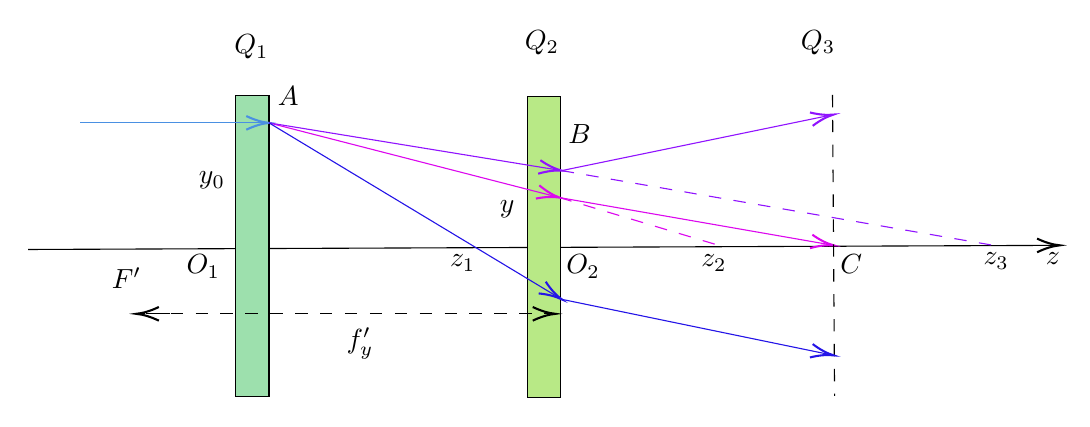
\begin{tikzpicture}[x=0.75pt,y=0.75pt,yscale=-1,xscale=1]
        %uncomment if require: \path (0,300); %set diagram left start at 0, and has height of 300
        
        %Straight Lines [id:da6447999895793526] 
        \draw    (85,148) -- (580,146.01) ;
        \draw [shift={(582,146)}, rotate = 179.77] [color={rgb, 255:red, 0; green, 0; blue, 0 }  ][line width=0.75]    (10.93,-3.29) .. controls (6.95,-1.4) and (3.31,-0.3) .. (0,0) .. controls (3.31,0.3) and (6.95,1.4) .. (10.93,3.29)   ;
        %Shape: Rectangle [id:dp18988569438393355] 
        \draw  [fill={rgb, 255:red, 157; green, 224; blue, 173 }  ,fill opacity=1 ] (185,74) -- (201,74) -- (201,219) -- (185,219) -- cycle ;
        %Straight Lines [id:da6543479198859878] 
        \draw [color={rgb, 255:red, 74; green, 144; blue, 226 }  ,draw opacity=1 ]   (110,87) -- (199,87) ;
        \draw [shift={(201,87)}, rotate = 180] [color={rgb, 255:red, 74; green, 144; blue, 226 }  ,draw opacity=1 ][line width=0.75]    (10.93,-3.29) .. controls (6.95,-1.4) and (3.31,-0.3) .. (0,0) .. controls (3.31,0.3) and (6.95,1.4) .. (10.93,3.29)   ;
        %Shape: Rectangle [id:dp25734994886242024] 
        \draw  [fill={rgb, 255:red, 184; green, 233; blue, 134 }  ,fill opacity=1 ] (325.5,74.5) -- (341.5,74.5) -- (341.5,219.5) -- (325.5,219.5) -- cycle ;
        %Straight Lines [id:da1255986891627514] 
        \draw  [dash pattern={on 4.5pt off 4.5pt}]  (141.59,179) -- (337,179) ;
        \draw [shift={(339,179)}, rotate = 180] [color={rgb, 255:red, 0; green, 0; blue, 0 }  ][line width=0.75]    (10.93,-3.29) .. controls (6.95,-1.4) and (3.31,-0.3) .. (0,0) .. controls (3.31,0.3) and (6.95,1.4) .. (10.93,3.29)   ;
        %Straight Lines [id:da8221720125141947] 
        \draw  [dash pattern={on 4.5pt off 4.5pt}]  (153.4,179) -- (139,179) ;
        \draw [shift={(137,179)}, rotate = 360] [color={rgb, 255:red, 0; green, 0; blue, 0 }  ][line width=0.75]    (10.93,-3.29) .. controls (6.95,-1.4) and (3.31,-0.3) .. (0,0) .. controls (3.31,0.3) and (6.95,1.4) .. (10.93,3.29)   ;
        
        %Straight Lines [id:da7104024027984699] 
        \draw [color={rgb, 255:red, 220; green, 8; blue, 238 }  ,draw opacity=1 ]   (201,87) -- (339.06,122.5) ;
        \draw [shift={(341,123)}, rotate = 194.42] [color={rgb, 255:red, 220; green, 8; blue, 238 }  ,draw opacity=1 ][line width=0.75]    (10.93,-3.29) .. controls (6.95,-1.4) and (3.31,-0.3) .. (0,0) .. controls (3.31,0.3) and (6.95,1.4) .. (10.93,3.29)   ;
        %Straight Lines [id:da42753255872189344] 
        \draw [color={rgb, 255:red, 220; green, 8; blue, 238 }  ,draw opacity=1 ]   (341,123) -- (471.03,145.66) ;
        \draw [shift={(473,146)}, rotate = 189.88] [color={rgb, 255:red, 220; green, 8; blue, 238 }  ,draw opacity=1 ][line width=0.75]    (10.93,-3.29) .. controls (6.95,-1.4) and (3.31,-0.3) .. (0,0) .. controls (3.31,0.3) and (6.95,1.4) .. (10.93,3.29)   ;
        %Straight Lines [id:da3584533349746679] 
        \draw [color={rgb, 255:red, 220; green, 8; blue, 238 }  ,draw opacity=1 ] [dash pattern={on 4.5pt off 4.5pt}]  (341,123) -- (421,147) ;
        %Straight Lines [id:da9006686803718542] 
        \draw  [dash pattern={on 4.5pt off 4.5pt}]  (472.5,73.5) -- (473.5,218.5) ;
        %Straight Lines [id:da4958481561557888] 
        \draw [color={rgb, 255:red, 144; green, 19; blue, 254 }  ,draw opacity=1 ]   (201,87) -- (340.03,109.68) ;
        \draw [shift={(342,110)}, rotate = 189.26] [color={rgb, 255:red, 144; green, 19; blue, 254 }  ,draw opacity=1 ][line width=0.75]    (10.93,-3.29) .. controls (6.95,-1.4) and (3.31,-0.3) .. (0,0) .. controls (3.31,0.3) and (6.95,1.4) .. (10.93,3.29)   ;
        %Straight Lines [id:da31749675107656694] 
        \draw [color={rgb, 255:red, 144; green, 19; blue, 254 }  ,draw opacity=1 ] [dash pattern={on 4.5pt off 4.5pt}]  (342,110) -- (550,146) ;
        %Straight Lines [id:da2533371967478151] 
        \draw [color={rgb, 255:red, 144; green, 19; blue, 254 }  ,draw opacity=1 ]   (342,110) -- (471.04,83.4) ;
        \draw [shift={(473,83)}, rotate = 168.35] [color={rgb, 255:red, 144; green, 19; blue, 254 }  ,draw opacity=1 ][line width=0.75]    (10.93,-3.29) .. controls (6.95,-1.4) and (3.31,-0.3) .. (0,0) .. controls (3.31,0.3) and (6.95,1.4) .. (10.93,3.29)   ;
        %Straight Lines [id:da24055375719244254] 
        \draw [color={rgb, 255:red, 36; green, 20; blue, 231 }  ,draw opacity=1 ]   (201,87) -- (340.29,170.97) ;
        \draw [shift={(342,172)}, rotate = 211.08] [color={rgb, 255:red, 36; green, 20; blue, 231 }  ,draw opacity=1 ][line width=0.75]    (10.93,-3.29) .. controls (6.95,-1.4) and (3.31,-0.3) .. (0,0) .. controls (3.31,0.3) and (6.95,1.4) .. (10.93,3.29)   ;
        %Straight Lines [id:da2184164871655463] 
        \draw [color={rgb, 255:red, 36; green, 20; blue, 231 }  ,draw opacity=1 ]   (342,172) -- (471.04,198.6) ;
        \draw [shift={(473,199)}, rotate = 191.65] [color={rgb, 255:red, 36; green, 20; blue, 231 }  ,draw opacity=1 ][line width=0.75]    (10.93,-3.29) .. controls (6.95,-1.4) and (3.31,-0.3) .. (0,0) .. controls (3.31,0.3) and (6.95,1.4) .. (10.93,3.29)   ;
        
        % Text Node
        \draw (574,148.4) node [anchor=north west][inner sep=0.75pt]    {$z$};
        % Text Node
        \draw (237.12,184.58) node [anchor=north west][inner sep=0.75pt]    {$f'_{y}$};
        % Text Node
        \draw (166,109.4) node [anchor=north west][inner sep=0.75pt]    {$y_{0}$};
        % Text Node
        \draw (311,123.4) node [anchor=north west][inner sep=0.75pt]    {$y$};
        % Text Node
        \draw (160,149.4) node [anchor=north west][inner sep=0.75pt]    {$O_{1}$};
        % Text Node
        \draw (204,68.4) node [anchor=north west][inner sep=0.75pt]    {$A$};
        % Text Node
        \draw (183,43.4) node [anchor=north west][inner sep=0.75pt]    {$Q_{1}$};
        % Text Node
        \draw (323,41.4) node [anchor=north west][inner sep=0.75pt]    {$Q_{2}$};
        % Text Node
        \draw (456,41.4) node [anchor=north west][inner sep=0.75pt]    {$Q_{3}$};
        % Text Node
        \draw (343,149.4) node [anchor=north west][inner sep=0.75pt]    {$O_{2}$};
        % Text Node
        \draw (344,86.4) node [anchor=north west][inner sep=0.75pt]    {$B$};
        % Text Node
        \draw (475,149.4) node [anchor=north west][inner sep=0.75pt]    {$C$};
        % Text Node
        \draw (124,155.4) node [anchor=north west][inner sep=0.75pt]    {$F'$};
        % Text Node
        \draw (287,149.4) node [anchor=north west][inner sep=0.75pt]    {$z_{1}$};
        % Text Node
        \draw (408,149.4) node [anchor=north west][inner sep=0.75pt]    {$z_{2}$};
        % Text Node
        \draw (544,148.4) node [anchor=north west][inner sep=0.75pt]    {$z_{3}$};
        
        
        \end{tikzpicture}
        } \\
        \caption{Các trường hợp về đường đi của tia sáng trên mặt phẳng $yOz$}
        \label{fig:45}
        \end{figure}

    Khi đã có được $f$ thỏa điều kiện, ta đi tìm tiêu cự $f'_y$ của thấu kính $Q_2$. Vẽ đường đi của tia sáng như hình \ref{fig:46} (để vẽ được hình, đầu tiên ta vẽ tia ló từ $Q_1$ $AB$ sao cho đường kéo dài của nó giao với trục chính tại tiêu điểm $F$ nằm trong đoạn $O_2 C$, sau đó nối điểm $B$ và $C$ lại rồi vẽ đường kéo dài của đoạn $BC$. Vẽ một trục phụ $\Delta$ song song với $AB$, giao của đường kéo dài $BC$ và $\Delta$ sẽ là $P$. Hạ $P$ vuông góc xuống trục chính, ta sẽ có được tiêu điểm $F'$ của thấu kính $Q_2$).
    
    \begin{figure}[!ht]
        \centering
        \scalebox{0.9}{
        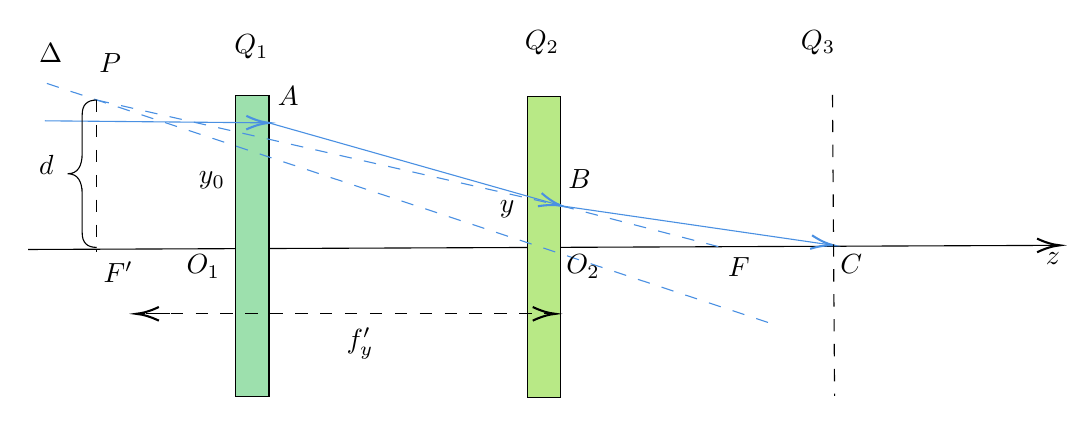
\begin{tikzpicture}[x=0.75pt,y=0.75pt,yscale=-1,xscale=1]
        %uncomment if require: \path (0,300); %set diagram left start at 0, and has height of 300
        
        %Straight Lines [id:da5591385678170064] 
        \draw    (85,148) -- (580,146.01) ;
        \draw [shift={(582,146)}, rotate = 179.77] [color={rgb, 255:red, 0; green, 0; blue, 0 }  ][line width=0.75]    (10.93,-3.29) .. controls (6.95,-1.4) and (3.31,-0.3) .. (0,0) .. controls (3.31,0.3) and (6.95,1.4) .. (10.93,3.29)   ;
        %Shape: Rectangle [id:dp029353147131552237] 
        \draw  [fill={rgb, 255:red, 157; green, 224; blue, 173 }  ,fill opacity=1 ] (185,74) -- (201,74) -- (201,219) -- (185,219) -- cycle ;
        %Straight Lines [id:da05730563683725465] 
        \draw [color={rgb, 255:red, 74; green, 144; blue, 226 }  ,draw opacity=1 ]   (93,86) -- (199,86.98) ;
        \draw [shift={(201,87)}, rotate = 180.53] [color={rgb, 255:red, 74; green, 144; blue, 226 }  ,draw opacity=1 ][line width=0.75]    (10.93,-3.29) .. controls (6.95,-1.4) and (3.31,-0.3) .. (0,0) .. controls (3.31,0.3) and (6.95,1.4) .. (10.93,3.29)   ;
        %Shape: Rectangle [id:dp3566188003815054] 
        \draw  [fill={rgb, 255:red, 184; green, 233; blue, 134 }  ,fill opacity=1 ] (325.5,74.5) -- (341.5,74.5) -- (341.5,219.5) -- (325.5,219.5) -- cycle ;
        %Straight Lines [id:da29781612172428007] 
        \draw  [dash pattern={on 4.5pt off 4.5pt}]  (141.59,179) -- (337,179) ;
        \draw [shift={(339,179)}, rotate = 180] [color={rgb, 255:red, 0; green, 0; blue, 0 }  ][line width=0.75]    (10.93,-3.29) .. controls (6.95,-1.4) and (3.31,-0.3) .. (0,0) .. controls (3.31,0.3) and (6.95,1.4) .. (10.93,3.29)   ;
        %Straight Lines [id:da7364739571960708] 
        \draw  [dash pattern={on 4.5pt off 4.5pt}]  (153.4,179) -- (139,179) ;
        \draw [shift={(137,179)}, rotate = 360] [color={rgb, 255:red, 0; green, 0; blue, 0 }  ][line width=0.75]    (10.93,-3.29) .. controls (6.95,-1.4) and (3.31,-0.3) .. (0,0) .. controls (3.31,0.3) and (6.95,1.4) .. (10.93,3.29)   ;
        
        %Straight Lines [id:da4177215727316572] 
        \draw [color={rgb, 255:red, 74; green, 144; blue, 226 }  ,draw opacity=1 ]   (201,87) -- (340.08,126.45) ;
        \draw [shift={(342,127)}, rotate = 195.84] [color={rgb, 255:red, 74; green, 144; blue, 226 }  ,draw opacity=1 ][line width=0.75]    (10.93,-3.29) .. controls (6.95,-1.4) and (3.31,-0.3) .. (0,0) .. controls (3.31,0.3) and (6.95,1.4) .. (10.93,3.29)   ;
        %Straight Lines [id:da6028751880008387] 
        \draw [color={rgb, 255:red, 74; green, 144; blue, 226 }  ,draw opacity=1 ]   (342,127) -- (471.02,145.71) ;
        \draw [shift={(473,146)}, rotate = 188.25] [color={rgb, 255:red, 74; green, 144; blue, 226 }  ,draw opacity=1 ][line width=0.75]    (10.93,-3.29) .. controls (6.95,-1.4) and (3.31,-0.3) .. (0,0) .. controls (3.31,0.3) and (6.95,1.4) .. (10.93,3.29)   ;
        %Straight Lines [id:da04563700924233949] 
        \draw [color={rgb, 255:red, 74; green, 144; blue, 226 }  ,draw opacity=1 ] [dash pattern={on 4.5pt off 4.5pt}]  (342,127) -- (419,147) ;
        %Straight Lines [id:da5223004912512463] 
        \draw [color={rgb, 255:red, 74; green, 144; blue, 226 }  ,draw opacity=1 ] [dash pattern={on 4.5pt off 4.5pt}]  (94,68) -- (444,184) ;
        %Straight Lines [id:da6250336384870441] 
        \draw [color={rgb, 255:red, 74; green, 144; blue, 226 }  ,draw opacity=1 ] [dash pattern={on 4.5pt off 4.5pt}]  (118,76) -- (342,127) ;
        %Shape: Brace [id:dp6416550287774179] 
        \draw   (118,76) .. controls (113.33,76) and (111,78.33) .. (111,83) -- (111,101.5) .. controls (111,108.17) and (108.67,111.5) .. (104,111.5) .. controls (108.67,111.5) and (111,114.83) .. (111,121.5)(111,118.5) -- (111,140) .. controls (111,144.67) and (113.33,147) .. (118,147) ;
        %Straight Lines [id:da9068429378811269] 
        \draw [color={rgb, 255:red, 0; green, 0; blue, 0 }  ,draw opacity=1 ] [dash pattern={on 4.5pt off 4.5pt}]  (118,76) -- (118,149) ;
        %Straight Lines [id:da7257837932260847] 
        \draw  [dash pattern={on 4.5pt off 4.5pt}]  (472.5,73.5) -- (473.5,218.5) ;
        
        % Text Node
        \draw (574,148.4) node [anchor=north west][inner sep=0.75pt]    {$z$};
        % Text Node
        \draw (237.12,184.58) node [anchor=north west][inner sep=0.75pt]    {$f'_{y}$};
        % Text Node
        \draw (166,109.4) node [anchor=north west][inner sep=0.75pt]    {$y_{0}$};
        % Text Node
        \draw (311,123.4) node [anchor=north west][inner sep=0.75pt]    {$y$};
        % Text Node
        \draw (160,149.4) node [anchor=north west][inner sep=0.75pt]    {$O_{1}$};
        % Text Node
        \draw (204,68.4) node [anchor=north west][inner sep=0.75pt]    {$A$};
        % Text Node
        \draw (183,43.4) node [anchor=north west][inner sep=0.75pt]    {$Q_{1}$};
        % Text Node
        \draw (323,41.4) node [anchor=north west][inner sep=0.75pt]    {$Q_{2}$};
        % Text Node
        \draw (456,41.4) node [anchor=north west][inner sep=0.75pt]    {$Q_{3}$};
        % Text Node
        \draw (343,149.4) node [anchor=north west][inner sep=0.75pt]    {$O_{2}$};
        % Text Node
        \draw (421,150.4) node [anchor=north west][inner sep=0.75pt]    {$F$};
        % Text Node
        \draw (89,101.4) node [anchor=north west][inner sep=0.75pt]    {$d$};
        % Text Node
        \draw (118,52.4) node [anchor=north west][inner sep=0.75pt]    {$P$};
        % Text Node
        \draw (344,108.4) node [anchor=north west][inner sep=0.75pt]    {$B$};
        % Text Node
        \draw (475,149.4) node [anchor=north west][inner sep=0.75pt]    {$C$};
        % Text Node
        \draw (120,152.4) node [anchor=north west][inner sep=0.75pt]    {$F'$};
        % Text Node
        \draw (89,47.4) node [anchor=north west][inner sep=0.75pt]    {$\Delta $};
        
        
        \end{tikzpicture}
        } \\
        \caption{Đường đi của tia sáng trên mặt phẳng $yOz$}
        \label{fig:46}
        \end{figure}
    $\Delta PF'O_2$ đồng dạng với $\Delta AO_1F$ nên:
    
    \begin{equation}
        \frac{y_0}{f} = \frac{d}{f'_y}
        \iff d = \frac{f'_y}{f}y_0.
    \end{equation}
    
    $\Delta BO_2C$ đồng dạng với $\Delta AO_1F$ nên:

    \begin{equation}
        \frac{|y|}{L} = \frac{d}{f'_y+L}
        \iff \frac{y_0}{f} (f-L) (f'_y + L) = \frac{y_0}{f} f'_y L
        \iff f'_y = \frac{L(f-L)}{2L-f}.
        \label{eq:42}
    \end{equation}
%hơi tắt, nên xét thêm ∆BFO_2 và ∆FPF' nữa.
    Ở đây, ta có thể thấy rằng $f'_y$ là độ lớn của tiêu cự nên để xác định thì $f'_y > 0$. Nhìn vào kết quả, ta thấy với $L < f < 2L$ thì $f'_y$ mới xác định, giống như điều kiện ban đầu ta lập ra cho $f$.

    Tương tự với mặt phẳng $xOz$, vẽ đường đi của tia sáng như hình \ref{fig:47}.

    \begin{figure}[!ht]
        \centering
        \scalebox{0.9}{
        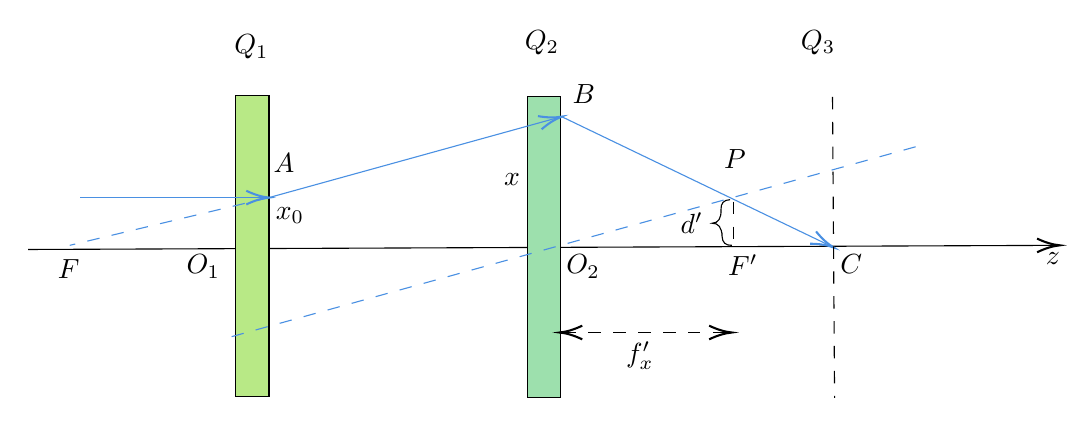
\begin{tikzpicture}[x=0.75pt,y=0.75pt,yscale=-1,xscale=1]
        %uncomment if require: \path (0,300); %set diagram left start at 0, and has height of 300
        
        %Straight Lines [id:da9134938091166365] 
        \draw    (85,148) -- (580,146.01) ;
        \draw [shift={(582,146)}, rotate = 179.77] [color={rgb, 255:red, 0; green, 0; blue, 0 }  ][line width=0.75]    (10.93,-3.29) .. controls (6.95,-1.4) and (3.31,-0.3) .. (0,0) .. controls (3.31,0.3) and (6.95,1.4) .. (10.93,3.29)   ;
        %Shape: Rectangle [id:dp8122623656554404] 
        \draw  [fill={rgb, 255:red, 184; green, 233; blue, 134 }  ,fill opacity=1 ] (185,74) -- (201,74) -- (201,219) -- (185,219) -- cycle ;
        %Straight Lines [id:da5355811934880252] 
        \draw [color={rgb, 255:red, 74; green, 144; blue, 226 }  ,draw opacity=1 ]   (110,123) -- (199,123) ;
        \draw [shift={(201,123)}, rotate = 180] [color={rgb, 255:red, 74; green, 144; blue, 226 }  ,draw opacity=1 ][line width=0.75]    (10.93,-3.29) .. controls (6.95,-1.4) and (3.31,-0.3) .. (0,0) .. controls (3.31,0.3) and (6.95,1.4) .. (10.93,3.29)   ;
        %Shape: Rectangle [id:dp6342039495818252] 
        \draw  [fill={rgb, 255:red, 157; green, 224; blue, 173 }  ,fill opacity=1 ] (325.5,74.5) -- (341.5,74.5) -- (341.5,219.5) -- (325.5,219.5) -- cycle ;
        %Straight Lines [id:da041957126485986374] 
        \draw  [dash pattern={on 4.5pt off 4.5pt}]  (342.89,188) -- (422,188) ;
        \draw [shift={(424,188)}, rotate = 180] [color={rgb, 255:red, 0; green, 0; blue, 0 }  ][line width=0.75]    (10.93,-3.29) .. controls (6.95,-1.4) and (3.31,-0.3) .. (0,0) .. controls (3.31,0.3) and (6.95,1.4) .. (10.93,3.29)   ;
        %Straight Lines [id:da5895401051908058] 
        \draw  [dash pattern={on 4.5pt off 4.5pt}]  (347.74,188) -- (343,188) ;
        \draw [shift={(341,188)}, rotate = 360] [color={rgb, 255:red, 0; green, 0; blue, 0 }  ][line width=0.75]    (10.93,-3.29) .. controls (6.95,-1.4) and (3.31,-0.3) .. (0,0) .. controls (3.31,0.3) and (6.95,1.4) .. (10.93,3.29)   ;
        
        %Straight Lines [id:da5087415687024939] 
        \draw [color={rgb, 255:red, 74; green, 144; blue, 226 }  ,draw opacity=1 ]   (201,123) -- (340.07,84.53) ;
        \draw [shift={(342,84)}, rotate = 164.54] [color={rgb, 255:red, 74; green, 144; blue, 226 }  ,draw opacity=1 ][line width=0.75]    (10.93,-3.29) .. controls (6.95,-1.4) and (3.31,-0.3) .. (0,0) .. controls (3.31,0.3) and (6.95,1.4) .. (10.93,3.29)   ;
        %Straight Lines [id:da3388874760521412] 
        \draw [color={rgb, 255:red, 74; green, 144; blue, 226 }  ,draw opacity=1 ]   (342,84) -- (471.2,146.13) ;
        \draw [shift={(473,147)}, rotate = 205.68] [color={rgb, 255:red, 74; green, 144; blue, 226 }  ,draw opacity=1 ][line width=0.75]    (10.93,-3.29) .. controls (6.95,-1.4) and (3.31,-0.3) .. (0,0) .. controls (3.31,0.3) and (6.95,1.4) .. (10.93,3.29)   ;
        %Straight Lines [id:da8510002260085452] 
        \draw [color={rgb, 255:red, 74; green, 144; blue, 226 }  ,draw opacity=1 ] [dash pattern={on 4.5pt off 4.5pt}]  (183,190) -- (518,97) ;
        %Straight Lines [id:da8211328953904067] 
        \draw [color={rgb, 255:red, 74; green, 144; blue, 226 }  ,draw opacity=1 ] [dash pattern={on 4.5pt off 4.5pt}]  (201,123) -- (105,146) ;
        %Shape: Brace [id:dp2484165614438989] 
        \draw   (423.13,124) .. controls (420.11,124.12) and (418.66,125.69) .. (418.78,128.71) -- (418.78,128.71) .. controls (418.95,133.02) and (417.53,135.24) .. (414.51,135.36) .. controls (417.53,135.24) and (419.12,137.34) .. (419.29,141.65)(419.22,139.71) -- (419.29,141.65) .. controls (419.41,144.67) and (420.98,146.12) .. (424,146) ;
        %Straight Lines [id:da7156522941896173] 
        \draw [color={rgb, 255:red, 0; green, 0; blue, 0 }  ,draw opacity=1 ] [dash pattern={on 4.5pt off 4.5pt}]  (425,125) -- (425,145) ;
        %Straight Lines [id:da7097487598870831] 
        \draw  [dash pattern={on 4.5pt off 4.5pt}]  (472.5,74.5) -- (473.5,219.5) ;
        
        % Text Node
        \draw (574,148.4) node [anchor=north west][inner sep=0.75pt]    {$z$};
        % Text Node
        \draw (371.81,191.02) node [anchor=north west][inner sep=0.75pt]    {$f'_{x}$};
        % Text Node
        \draw (203,126.4) node [anchor=north west][inner sep=0.75pt]    {$x_{0}$};
        % Text Node
        \draw (313,110.4) node [anchor=north west][inner sep=0.75pt]    {$x$};
        % Text Node
        \draw (160,149.4) node [anchor=north west][inner sep=0.75pt]    {$O_{1}$};
        % Text Node
        \draw (202,100.4) node [anchor=north west][inner sep=0.75pt]    {$A$};
        % Text Node
        \draw (183,43.4) node [anchor=north west][inner sep=0.75pt]    {$Q_{1}$};
        % Text Node
        \draw (323,41.4) node [anchor=north west][inner sep=0.75pt]    {$Q_{2}$};
        % Text Node
        \draw (456,41.4) node [anchor=north west][inner sep=0.75pt]    {$Q_{3}$};
        % Text Node
        \draw (343,149.4) node [anchor=north west][inner sep=0.75pt]    {$O_{2}$};
        % Text Node
        \draw (421,149.4) node [anchor=north west][inner sep=0.75pt]    {$F'$};
        % Text Node
        \draw (398.07,128.84) node [anchor=north west][inner sep=0.75pt]    {$d'$};
        % Text Node
        \draw (346,67.4) node [anchor=north west][inner sep=0.75pt]    {$B$};
        % Text Node
        \draw (475,149.4) node [anchor=north west][inner sep=0.75pt]    {$C$};
        % Text Node
        \draw (98,151.4) node [anchor=north west][inner sep=0.75pt]    {$F$};
        % Text Node
        \draw (419,98.4) node [anchor=north west][inner sep=0.75pt]    {$P$};
        
        
        \end{tikzpicture}
        } \\
        \caption{Đường đi của tia sáng trên mặt phẳng $xOz$}
        \label{fig:47}
        \end{figure}
    $\Delta PF'O_2$ đồng dạng với $\Delta BO_2F$ nên:

    \begin{equation}
        \frac{d'}{f'_x}=\frac{x_0}{f}
        \iff d' = \frac{f'_x}{f}x_0.
    \end{equation}

    $\Delta PF'C$ đồng dạng với $\Delta BO_2C$ nên:

    \begin{equation}
        \frac{d'}{L-f'_x} = \frac{x}{L}
        \iff \frac{x_0}{f}(L+f)(L-f'_x) = \frac{x_0}{f}f'_xL
        \iff f'_x = \frac{L(f+L)}{2L+f}.
        \label{eq:43}
    \end{equation}
% cũng hơi tắt. Làm thêm một phương trình đồng dạng nữa.
    Tiêu cự của thấu kính $Q_2$ ở trên cả hai phương $x$ và $y$ đều bằng nhau nên từ (\ref{eq:42}) và (\ref{eq:43}) ta được:

    \begin{equation}
        f'_x = f'_y
        \iff \frac{L(f-L)}{2L-f} = \frac{L(f+L)}{2L+f}
        \iff f = \sqrt{2}L.
    \end{equation}

    \begin{equation}
        \Longrightarrow f'_x = f'_y = f' = \frac{L \left(\sqrt{2}L + L \right)}{2L + \sqrt{2}L} = \frac{L}{\sqrt{2}}.
    \end{equation}
    Tức $f = 2f'$.
    \end{enumerate}

    \item \textbf{Phổ điểm}
    
    \begin{center}
    \begin{tabular}{|c|p{8cm}|c|}
    \hline
    \multicolumn{1}{|l|}{Phần} & Nội dung & Điểm thành phần \\ 
    \hline
    1 & Xác định đúng phương và chiều của đường sức từ và lực điện từ & 0.50 \\
    \hline
    2 & Xác định tọa độ $x$ và $y$ của điểm B & 0.25/tọa độ \\
    \hline
    \multirow{2}{*}{3}         
    & Lập luận được các trường hợp về đường đi của tia sáng & 0.50 \\
    \cline{2-3} 
    & Xác định được điều kiện của $f$ & 0.50 \\
    \cline{2-3} 
    & Vẽ được hai hình \ref{fig:46} và \ref{fig:47} & 0.25/ảnh \\
    \cline{2-3}
    & Biểu diễn $f'_y$ theo $L$ & 0.50  \\
    \cline{2-3}
    & Biểu diễn $f'_x$ theo $L$ & 0.50  \\
    \cline{2-3}
    & Biểu diễn $f$ và $f'$ theo $L$  & 0.25/biểu thức \\
    \hline
    \end{tabular}
    \end{center}
    Lưu ý: Nếu suy ra điều kiện của $f$ từ phương trình (\ref{eq:42}) thì không được điểm phần lập luận. 
\end{enumerate}